This work makes use of probability meshes to approximate a 4-dimensional (position,velocity) space. The meshes are then used to implement efficient forward estimation, integration of new sensor data, and integration of probabilistic rules. Finally, a pipeline is constructed from these elements to produce refined paths from raw positional input.

\section{Probability Meshes}

Each trajectory of interest $t$ has an associated 4-dimensional $n*m*i*j$ probability mesh $M_t$, with each cell $M_t(n,m,i,j)$ in the mesh representing the likelihood that the most recent position and velocity in the trajectory lie in that cell.
However $n$, $m$, $i$, and $j$ are integer values while locations and velocities are continuous.
In order to account for continuous values, an interpolation scheme can approximate points between cell centers.

Interpolation works as follows: For each dimension $i$ in a query point $q=(q_n, q_m, q_i, q_j)$, calculate $\mathit{floor}(i)$ and $\mathit{ceil}(i)$. Then collect the set of adjacent points $P$ by generating all combinations of $floor$ and $ceil$ in each dimension. Interpolation is calculated over $P$ as shown in Equation \ref{eqn:interpolation}.

\begin{equation} \label{eqn:interpolation}
    \frac{\sum_{p \in P} 1/\mathit{dist}(p, q) * M_t(p_n, p_m, p_i, p_j)}{\sum_{p \in P} (1/\mathit{dist}(p, q)}
\end{equation}

With interpolation between cells, probability meshes can approximate a bounded continuous probability. Note that the division by \textit{dist} is undefined when dist is zero. In practice, that can only occur when all indices are integers, and in that case the exact point found is returned. This interpolation algorithm has a property that will be heavily utilized in the remainder of the paper: Because all probabilities are weighted by \textit{dist}, probabilities generated from a set of points are bounded by the minimum and maximum values stored in those points. Therefore, the point of maximum probability \textit{must be an exact grid cell}.

However, the grid indices have no mapping to real-world positions and velocities. To provide mappings, boundaries and a mapping function must be specified. Given an input position and velocity $(p_x, p_y, v_x, v_y)$ and boundaries $x_{min}, x_{max}, y_{min}, y_{max}, v_{min}, v_{max}$, the appropriate grid point is calculated by Equation \ref{eqn:normalize}.

\begin{equation} \label{eqn:normalize}
    \begin{aligned}
        map(p_x, p_y, v_x, v_y) = &\\
        (&\frac{(p_x - x_{min})*n}{x_{max}-x_{min}},\\
        &\frac{(p_y - y_{min})*m}{y_{max}-y_{min}}, \\
        &\frac{(v_x - v_{min})*i}{v_{max}-v_{min}},\\
        &\frac{(v_y - v_{min})*j}{v_{max}-v_{min}})
    \end{aligned}
\end{equation}

With the inclusion of the mapping function and boundaries, a probability mesh can approximate a continuous probability over arbitrary boundaries. In addition, the mapping function can be reversed to $map_{reverse}$, calculating the corresponding point in the probability space for a particular cell in the mesh.

\subsection{Forward Propagation}

Because these probability meshes capture both position and velocity, future probability spaces can be estimated. Equation \ref{eqn:timeprop} shows how a zeroed mesh $M_t'$ can be calculated from a past mesh $M_t$.

\begin{equation} \label{eqn:timeprop}
    M_t'(n+(t'-t)i,m+(t'-t)j,i,j) += M_t(n,m,i,j)
\end{equation}

$M_t'$ represents an accurate estimate, assuming unchanging velocities. However in the real world objects can change velocity over time. To accomodate this, a blur factor can be added by averaging all adjacent points using a stencil algorithm.

\section{Probabilistic Rules}

Often in addition to sensor input, we have domain knowledge about objects whose positions and velocities are being tracked. Such rules can often be colloquially expressed as "Cars tend to drive on roads", or "Trucks and busses rarely make U-turns". Under a traditional path refinement system such as a Kalman Filter, these rules cannot be expressed, as they represent non-gaussian probabilities. However, using probability meshes, these rules can be approximated and used to refine any sensor inputs or estimates. In order for a rule to help refine paths, it need not always be true. The examples above discuss things that usually occur, which can be formally defined as a probability. By phrasing rules as probability functions in the same 4-dimensional position, velocity space as the meshes defined above, such probabilistic rules can be expressed.

A rule $R$ can be intersected with a mesh $M$ by applying the pointwise update equation -- Equation \ref{eqn:ruleupdate} -- to all cells in the mesh, producing a new mesh $M'$. Multiplication allows the probabilities to be combined to generate the probability of both the original mesh and the rule being true for each cell.

\begin{equation} \label{eqn:ruleupdate}
    M'(n, m, i, j) = M(n, m, i, j) * R(map_{reverse}(n,m,i,j))
\end{equation}

\subsection{Road Matching}

As an example of probabilistic rules, this work implements the rule \textit{"vehicles usually drive on roads"}. The exact equation for this rule is in Equation \ref{eqn:roadprob}.

\begin{equation} \label{eqn:roadprob}
    \begin{gathered}
    R_{road}(p_x, p_y, v_x, v_y) = \\
        \textit{max}(\alpha, \textit{CNDF}(\textit{distanceToRoad}(p_x, p_y)/\beta))
    \end{gathered}
\end{equation}

$\alpha$ allows for this rule being incorrect, by setting a lower bound on the probability of any cell, regardless of roadways. $\beta$ allows the allowed distance from the roadway to be scaled. Here CNDF refers to the cumulative normal distribution function, which returns a value between 0.5 and 0 for positive inputs.

The \textit{distanceToRoad} function requires additional explanation.
Road map data for the city of Edmonton was aquired from OpenStreetMap, and roadways were extracted. Then, to reduce the number of roadways inspected for a particular calculation of this rule, a uniform grid index is overlaid on the area of interest, and roads are placed into each grid cell overlapped by their minimum bounding rectangle~(MBR). Grid cells should be of a width substantially larger than $\beta$ above, so that a minimum of cells need to be inspected.

When calculating \textit{distanceToRoad} for a given point, all roads in the corresponding index cell are collected, as well as all roads in adjacent cells to account for query points near the edge of a cell. Then, the distance from each segment of each road to the query point is calculated. Finally, the minimum distance found is returned. An example of the probability space rendered from this work is shown in \figref{fig:ex:osm}.

\begin{figure}
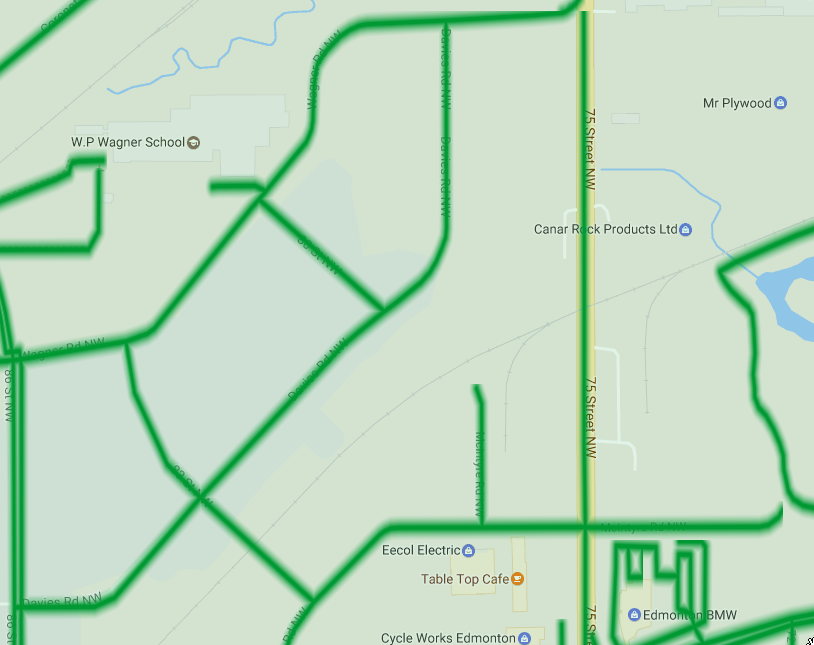
\includegraphics[scale=0.28]{figures/OSMRoadProb.png}
\caption{Example rule "Vehicles usually drive on roads" overlaid on Google Maps}
\label{fig:ex:osm}
\end{figure}


\section{Grid-Based Trajectory Refinement}

From probability meshes and probabilistic rules, a pipeline can be assembled to refine trajectories in real-time. Consider a set of objects being tracked, $O$.
Each object $o \in O$ has an associated probability mesh $M(o)$, valid for a particular timestamp in the past $updateTime(o)$. All probability meshes are initialized to an equal uniform distribution.
As each sensor update $(o, \mathit{time}, p_x, p_y)$ comes in, meshes are updated according to the following pipeline:

\begin{enumerate}

\item The object mesh is propagated forward in time according to Equation \ref{eqn:timeprop}, using the time difference $\textit{time} - \textit{updateTime}(o)$.

\item A gaussian probability $\textit{GPS}$ is constructed around $p_x, p_y$, constructed to match the error distribution that 95\% of sensor readings are within 2 meters of accurate. The GPS probability is integrated into $M(o)$ according to Equation \ref{eqn:ruleupdate}.

\item Any applicable rules can be integrated, again using Equation \ref{eqn:ruleupdate}.

\item The new most likely position is found by finding the maximum cell in mesh $M(o)$ and reverse mapping the cell into the real-world position.

\end{enumerate}


